\documentclass[12pt, twoside]{article}
\usepackage[letterpaper, margin=1in, headsep=0.5in]{geometry}
\usepackage[english]{babel}
\usepackage[utf8]{inputenc}
\usepackage{amsmath}
\usepackage{amsfonts}
\usepackage{amssymb}
\usepackage{tikz}
\usepackage{yhmath}
%\usetikzlibrary{quotes, angles}

\usepackage{graphicx}
\usepackage{enumitem}
\usepackage{multicol}

\usepackage{fancyhdr}
\pagestyle{fancy}
\fancyhf{}
\renewcommand{\headrulewidth}{0pt} % disable the underline of the header

\fancyhead[RE]{\thepage}
\fancyhead[RO]{\thepage \\ Name: \hspace{3cm}}
\fancyhead[L]{BECA / Dr. Huson / 10th Grade Geometry\\* 21 May 2019}

\begin{document}

\subsubsection*{Pop Re-Quiz: Density \& compound shapes}
\emph{You must show the calculation, as well as the result, for credit.}
 \begin{enumerate}

\item A candle has the shape of a cylinder. It is 9.25 inches tall and the diameter of its base is 4.5 inches. Find the volume of the candle to the \emph{nearest cubic inch}. \vspace{3cm}

\item A alabaster figurine has a volume of 670 cm$^3$. Find its weight, to the \emph{nearest tenth of a kilogram}. (assume the density of alabaster is $2.40 \ \mathrm{grams}/ \mathrm{cm}^3$) \vspace{3cm}

\item The area of Queens, NY is 108 square miles. Its population density is approximately 21,850 people per square mile. Estimate the population of Queens. \vspace{3cm}

\item The volume of a pyramid with a square base is found to be 356.25 using the formula:
  \[V=\frac{1}{3} x^2 \times 19=356.25\]
  What does the value $19$ in the formula represent? Solve for the length of the side of the square base. \vspace{4cm}

\newpage
\item BECA middle schoolers draw a basketball key on the asphalt in chalk. It is rectangular with one end round. It is 5 feet wide and overall it is $9 \frac{1}{2}$ feet long, as shown. Find the area of the chalked basketball key to the \emph{nearest square foot}.\\[1.5cm]
  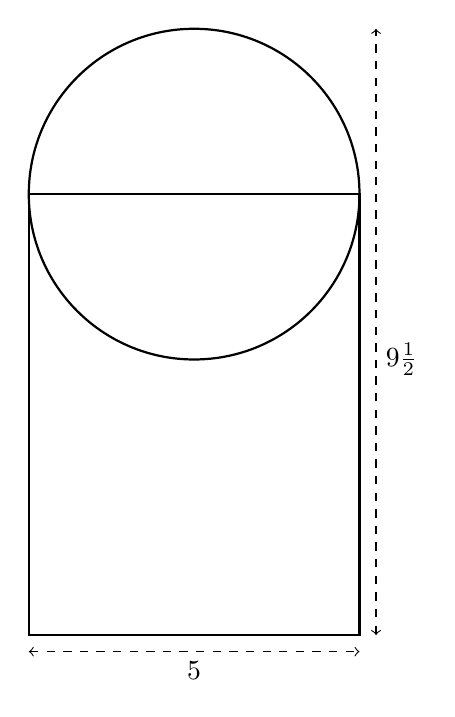
\begin{tikzpicture}[scale=0.7]
    \draw [thick]
    (0,0)--(0,8)--(6,8)--(6,0)--cycle;
    \draw [thick] (3,8) circle[radius=3];
    \draw [dashed,<->] (6.3,0)--(6.3,11);
    \draw [dashed,<->] (0,-0.3)--(6,-0.3);
    %\draw (0,8)++(0,-0.8)--++(0.8,0)--+(0,0.8);
    \node at (3,-0.3)[below]{$5$};
    \node at (6.3,5)[right]{$9 \frac{1}{2}$};
    %\node at (6.25,7)[right]{$2$};
  \end{tikzpicture}

\item A concrete ramp is poured to be level to an entryway. There are two steps leading to the entryway, each 10 inches tall. The length of the ramp is 10 feet. What is the angle of elevation, $x$, that the ramp makes to the ground, to the \emph{nearest degree}.\\[1.cm]
      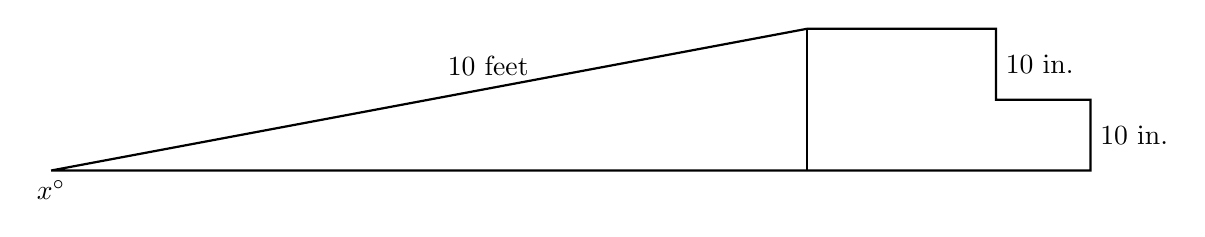
\begin{tikzpicture}[scale=0.6]
        \draw [thick] (-6,0)--(10,3)--(14,3)--(14,1.5)--(16,1.5)--(16,0)--cycle;
        \draw [thick] (10,0)--(10,3);
        %\draw (10,16)++(0,-0.8)--++(0.8,0)--+(0,0.8);
        \node at (16,0.75)[right]{$10 \ \mathrm{in.}$};
        \node at (14,2.25)[right]{$10 \ \mathrm{in.}$};
        \node at (-6,0)[below]{$x^\circ$};
        \node at (3.25, 1.8)[above]{$10 \ \mathrm{feet}$};
        %\node at (14, 4)[above]{\emph{Not to Scale}};
      \end{tikzpicture} \vspace{5cm}



  \end{enumerate}
  
\end{document}
